\documentclass[11pt]{article}
\usepackage{libertine}
\usepackage{tikz}

\title{{\em Modern Climate Change}: a cheat-sheet}
\begin{document}

\maketitle

\section{Introduction}
This doc is a collection of notes from the climate science chapters of the
book {\em Modern Climate Change} by Andrew Dessler. It's intended as a quick
reference for the main concepts and formulas for those who've read the book.

\section{Climate history}

\subsection{Recent history}

{\em Temperature anomalies} are the difference between an absolute temperature and a reference
temperature, typically the average temperature over a period of time.

Temperature anomalies can be measured using a network of thermometers that is sparser than
that needed to measure the absolute temperature. The global average temperature
anomaly can be measured using only about 100 thermometer stations. The surface thermometer
record must be adjusted for changes in measurement practices, environmental
changes such as urbanization, and changes in the instruments themselves.

Satellite measurements have been available since 1978. They also need to be adjusted for various
factors including orbital drift and the fact that they measure average atmospheric temperature,
not surface temperature.

The instrumental record shows that the Earth has warmed by about $1.1^\circ$C between the late
1800s and 2010.

Additional indirect evidence of recent climate change includes glacier and ice sheet retreat and
the shrinking of Arctic sea ice.

The top 2000 m of world oceans have warmed by about $0.12^\circ$C between 1960 and 2010.

Ice melt over land and thermal expansion of seawater have caused sea levels to rise by about 100 mm
between 1995 and 2020.

\subsection{Long-term climate record}

Climate data prior to the instrumental record can be obtained from several {\em paleoproxies}, including:

\begin{itemize}
    \item The chemical composition and crystal structure of ice cores.
    \item The chemical composition of air bubbles trapped in ice cores.
    \item Tree rings. (Trees grow more in warm climates.)
    \item Ocean sediments, and in particular the prevalance of different species and the chemical
        composition of the fossils.
\end{itemize}

In the last 400M years Earth has alternated between "icehouse" and "greenhouse" states.
During icehouse phases, ice has reached south to $30^\circ$ latitude. During greenhouse phases,
ice disappeared from the poles.

The last greenhouse phase ended about 35M years ago. The peak temperature occurred about 55M years ago,
with the Earth briefly $20^\circ$C warmer than today (Paleocen-Eocene Thermal Maximum).

Until about 3M years ago, temperatures cooled gradually. After that, large ice sheets appeared in the
Northern Hemisphere and oscilations between warm and cold periods appear in the record.

Between approximately 2.5M and 1M years ago, ice ages occured every 41K years. About 1M years ago,
the frequency changed to every 100K years and the amplitude of the temperature changes increased.

In the last 400K years, ice ages have lasted about 100K years and interglacials about 10-30K years.
Cooling took a long time (tens of thousands of years) but warming was rapid (about 10K years).

Atmospheric CO$_2$ concentration in ice cores tracks temperature changes closely.

\section{Radiation and energy balance}

\section{Simple climate models}
\[
T = \sqrt[4]{\frac{(n+1)S(1-\alpha)}{4 \sigma}}
\]


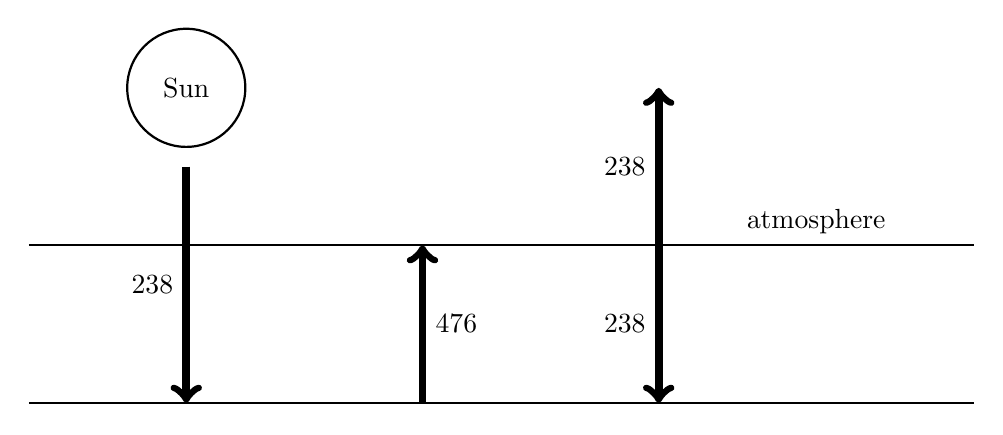
\begin{tikzpicture}[xscale=2]
    % Sun
    \node at (1,4) [circle, draw, thick, minimum size=1.5cm] {Sun};

    % Atmosphere layer
    \draw[thick] (0, 2) -- (6, 2);
    \node at (5, 2.3) {atmosphere};

    % Ground layer
    \draw[thick] (0, 0) -- (6, 0);

    % Arrows
    % sun to earth
    \draw[line width=1mm, ->] (1, 3) -- (1, 0) node[midway, left] {238};
    % earth to atmosphere
    \draw[line width=1mm, ->] (2.5, 0) -- (2.5, 2) node[midway, right] {476};

    % atmosphere to earth
    \draw[line width=1mm, ->] (4, 2) -- (4, 0) node[midway, left] {238};
    % atmosphere to space   
    \draw[line width=1mm, ->] (4, 2) -- (4, 4) node[midway, left] {238};

\end{tikzpicture}

\section{The carbon cycle}
\section{Forcings, feedbacks, and climate sensitivity}

\end{document}